\section{FaceLift Framework}
\label{sec:framework}

\begin{table}[t]
	\resizebox{\linewidth}{!}{
		\begin{tabular}{l|p{8cm}}
			\textbf{Symbol} & \textbf{Meaning}\\
			$I_i$    & Original urban scene \\
			$Y$    & Set of annotation classes for urban scenes (e.g., beautiful, ugly)\\
			$y_i$    & Annotation class in $Y$ (e.g., beautiful) \\
			$\hat{I_j}$ & Template scene (synthetic image) \\
			$I'$ & Target Image \\
			$C$ & Beauty Classifier \\
	\end{tabular}}
	\caption{Notations}\label{notations}
\end{table}

 \begin{figure*}[ht]
	\centering
	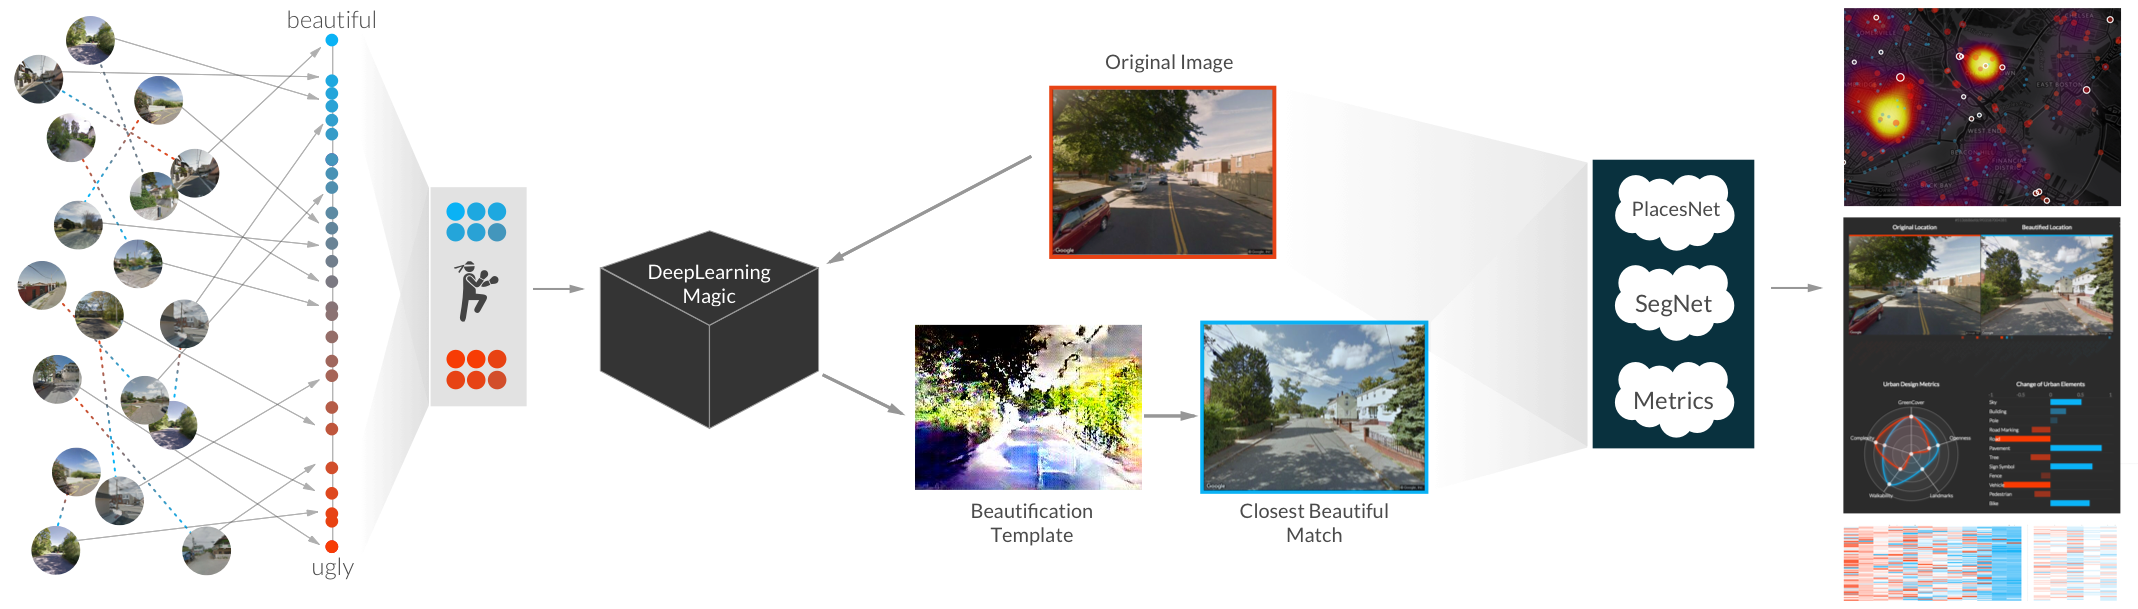
\includegraphics[width=\linewidth]{Plot/FaceLift.png}
	\caption{A simplistic end to end illustration of the FaceLift framework.}
	\label{fig:framework}
\end{figure*}

\begin{figure}[t!]
	\centering
	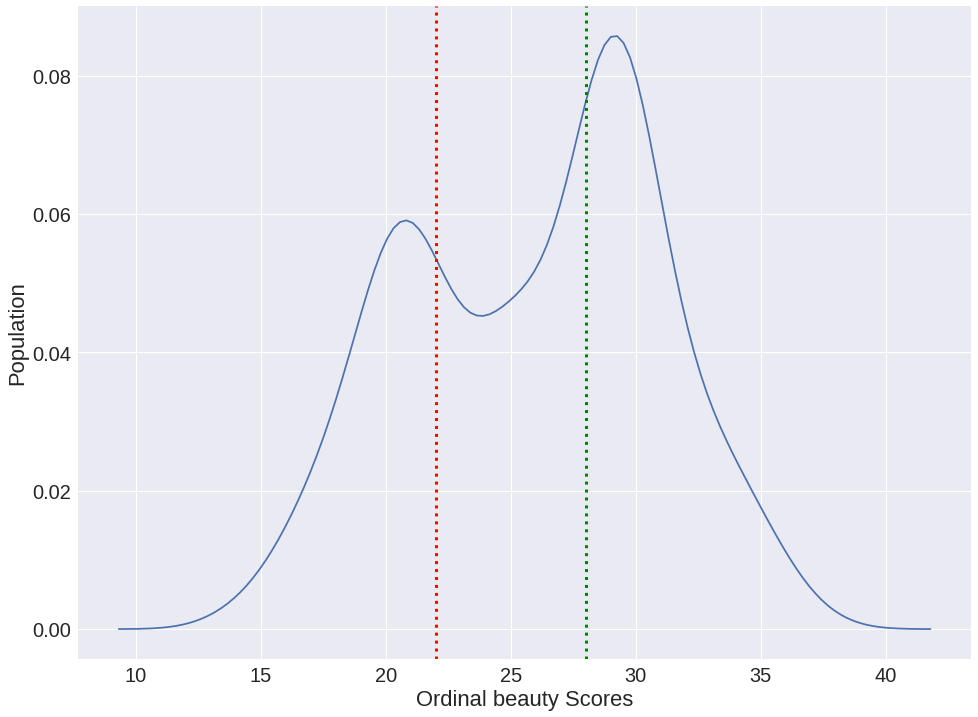
\includegraphics[width=0.7\columnwidth]{Plot/Trueskill.png}
	\caption{Frequency distribution of beauty scores. The red and green lines represent the thresholds below and above which images are considered ugly and beautiful. Conservatively, images in between are discarded.}
	\label{fig:Trueskill}
\end{figure}

%****************************************
The goal of FaceLift is to take as input a geo-located urban scene and give as output its transformed (beautified) version. 
To that end, it performs five steps: 1) curating urban scenes; 2) training a beauty classifier; 3) generating a synthetic beautified scene; 4) returning a realistic beautified scene; and 5) identifying the urban elements characterizing the beautified scene. 
 
 
 
\begin{figure*}[t!]
	\centering
	\hspace*{-5mm}
	\subfloat[]{
		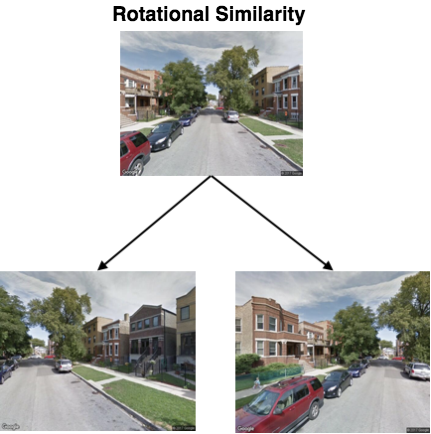
\includegraphics[width=0.5\textwidth, height = 8cm ]{Plot/rotationalSim.png}
		\label{fig:rotSim}
	}
	\subfloat[]{
		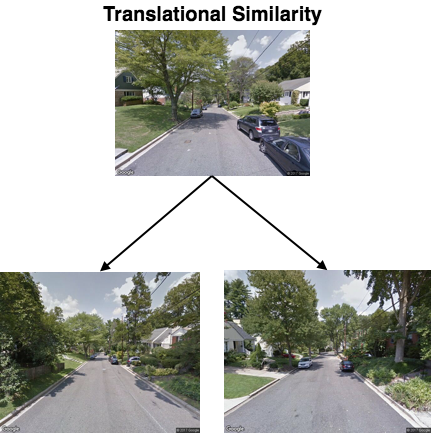
\includegraphics[width=0.5\linewidth, height = 8cm ]{Plot/transSim.png}
		\label{fig:transSim}
	}
	\vspace{-0.4cm}
	\caption{Two types of augmentation: (a) rotation of the Street Views camera (based on rotation); and (b) exploration of scenes at increasing distances (based on translation).}
	\vspace{-0.4cm}
\end{figure*}


%****************************************
\subsection*{Step 1 Curating Urban Scenes}
To begin with, we need highly curated training data with labels reflecting urban beauty. We start with the  Place Pulse dataset that contains 100k Google Street Views across 56 cities around the world~\cite{dubey2016deep}. These scenes are labeled in terms of whether the corresponding places are likely to be perceived beautiful, depressing, rich, and safe. We focus only on those scenes that are labeled in terms of beauty and that have at least three judgments. This leave us with roughly  20,000 scenes. To transform judgments into beauty scores, we use the TrueSkill algorithm~\cite{herbrich2007trueskill}, which gives us a way of partitioning the scenes into two sets (Figure \ref{fig:Trueskill}): one containing beautiful scenes, and the other containing ugly scenes. The resulting set of scenes is too small for training any deep learning module without avoiding over-fitting though. As such, we need to augment such a set. We do so in two ways. First, we feed each scene's location into the Google Streetview API to obtain  the snapshots of the same location at different camera angles (i.e., at $\theta \in {-30^{\circ}, -15^{\circ} , 15^{\circ} , 30^{\circ} }$). However, the resulting dataset is still too small for robust training. Therefore, again, we feed each scene's location into the Google Streetview API, but now we do so to obtain other scenes at  distance $d \in \{10,20,40,60\}$ meters.  This will greatly expand our set of scenes, but it might do so at the price of introducing scenes whose beauty scores have little to do with the original scene's. To fix that, we take only the scenes that are \emph{similar} to the original one (we call this way of augmenting ``conservative translation''). To compute the similarity between a pair of scenes, we represent the two scenes with visual features derived from the FC7 layer of PlacesNet and compute the similarity between the two corresponding feature vectors~\cite{zhou2014learning}. For all scenes at increasing distance $d \in \{10,20,40,60\}$ meters,  we take only those whose similarity scores with the original scene is above a threshold. In a conservative fashion, we choose that threshold to be the median similarity between rotated and original scenes (those of the first augmentation step). To make sure this additional augmentation has not introduced any unwanted noise, we consider  two sets of scenes: one containing those that have been taken during this last step (\emph{taken-set}), and the other containing those that have been filtered away (\emph{filtered-set}). Each scene is labeled with PlacesNet~\cite{zhou2014learning} and is represented with the five most confident scene labels. The labels are aggregated  at set level by computing each label's frequency on the \emph{taken-set} minus that on the \emph{filtered-set} and by then characterizing each label's propensity to be correctly augmented as: 
$ \textrm{prone}(label)= fr(label,\textrm{\emph{taken-set}}) - fr(label,\textrm{\emph{filtered-set}}).$
This reflects the extent to which a scene with a given label is prone to be augmented or not. From Figure~\ref{fig:augmentationSimilarity}, we find that, as one would expect, scenes that contain highways, fields and bridges can be augmented at increasing distances while still showing resemblances to the original scene; by contrast, scenes that contain gardens, residential neighbourhoods , plazas, and skyscrapers cannot be easily augmented, as they are often found in high density parts of the city.


\begin{figure}[t!]
	\centering
	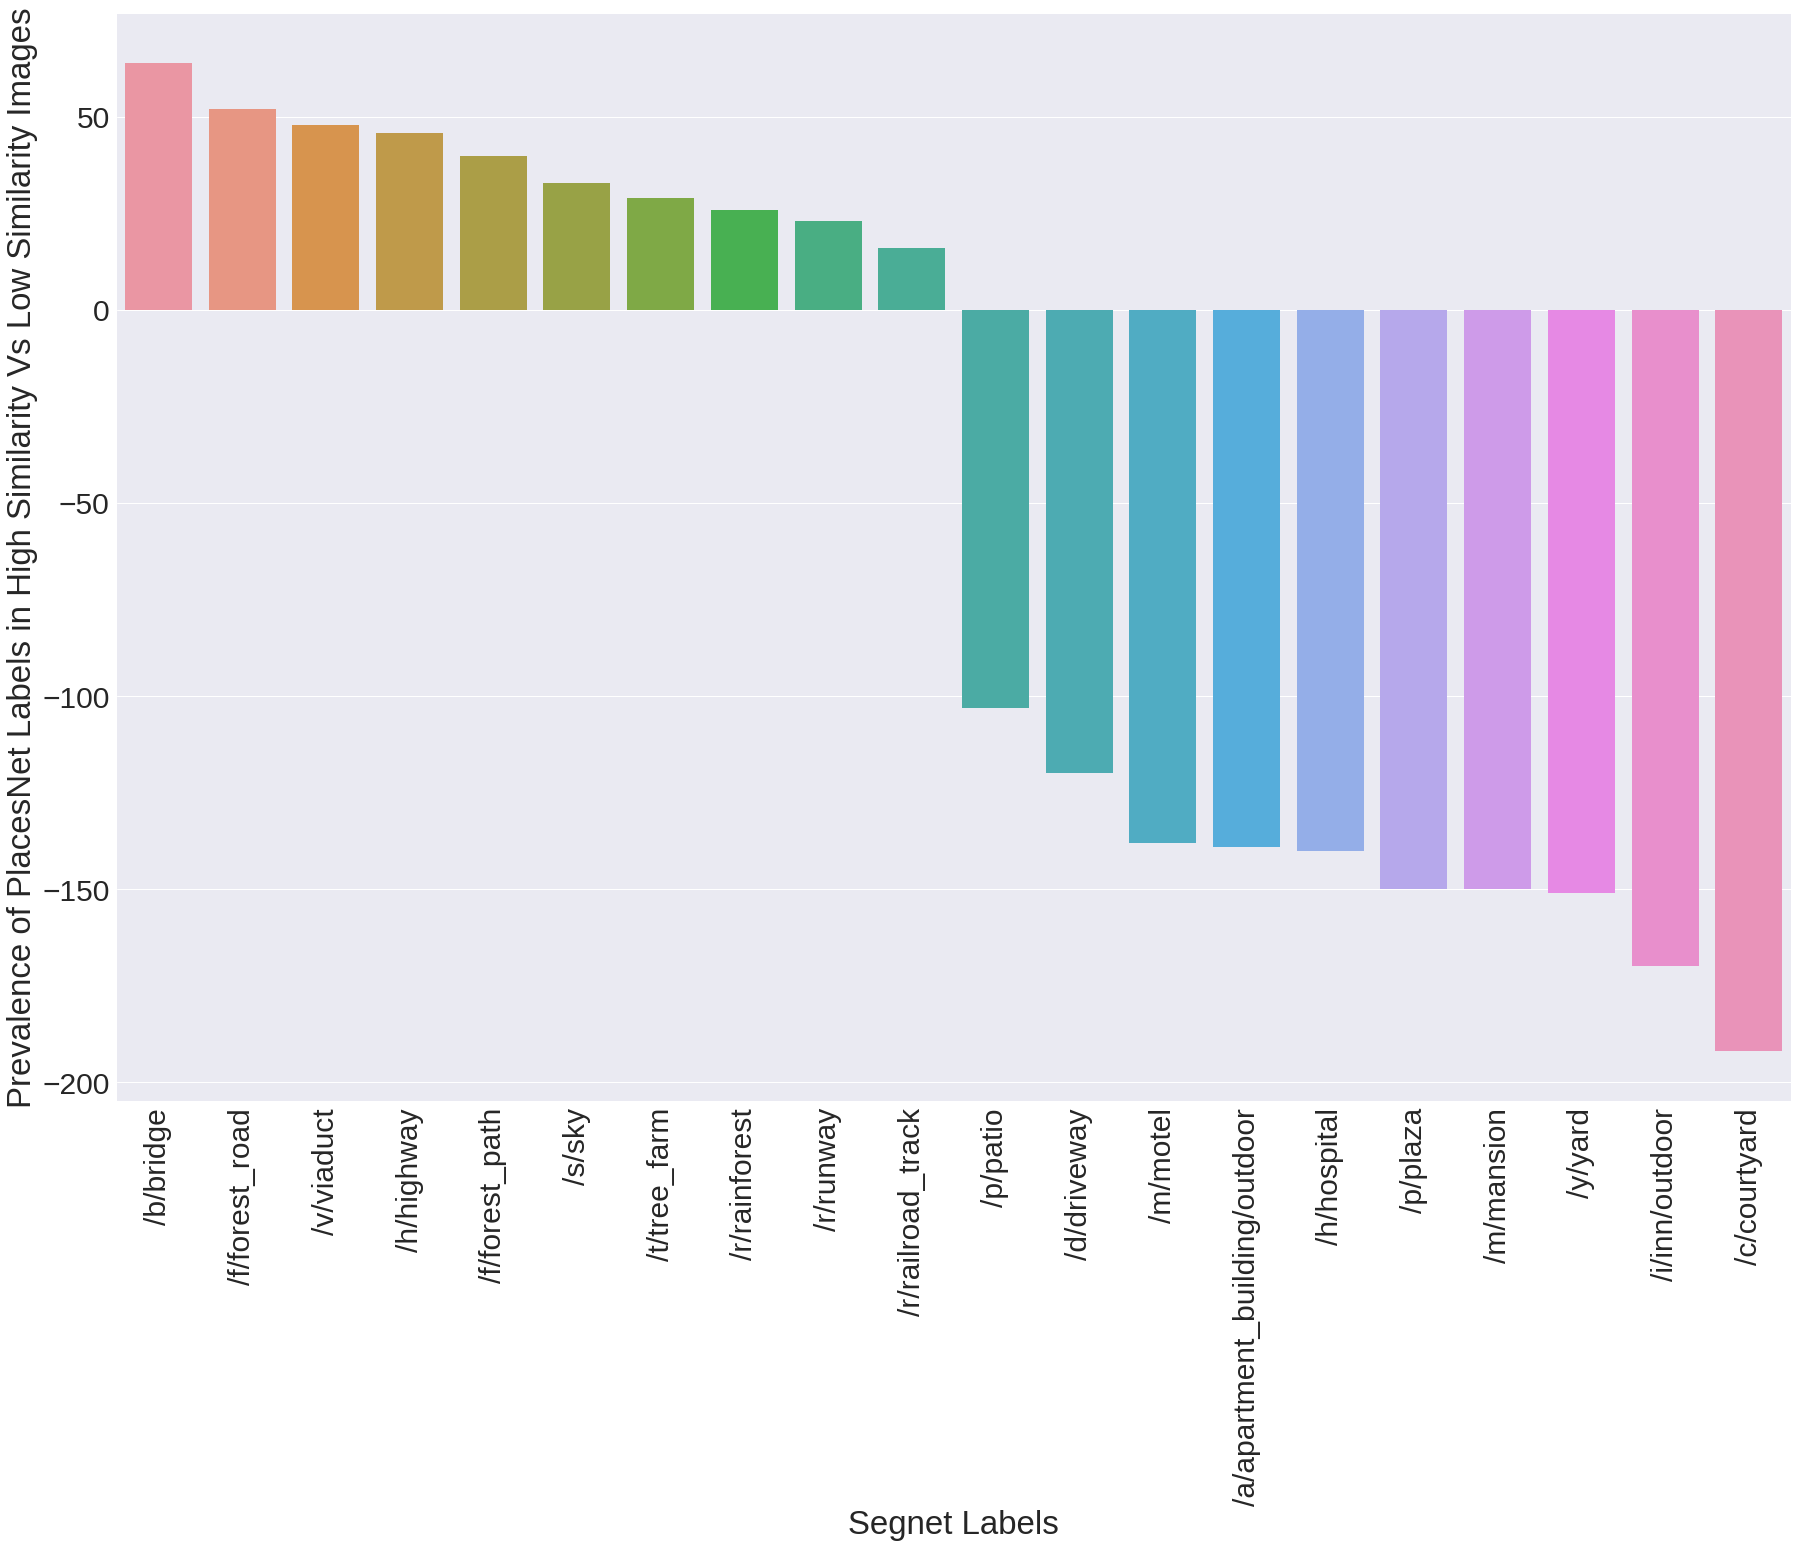
\includegraphics[width=\columnwidth]{Plot/SimilarityPlacesPrevalence.png}
	\caption{The types of scene that have greater propensity to be correctly augmented with similar scenes at increasing distances.}
	\label{fig:augmentationSimilarity}
\end{figure}




\begin{table}[t!]
	\centering
	\begin{tabular}{|c|c|}
		\hline
		\textbf{Augmentation} & \textbf{Accuracy (Percentage)}\\
		\hline
		None & 63 \\
		\hline
		Rotation  & 68 \\
		\hline
		Rotation + Translation  & 64 \\
		\hline
		Rotation + Conservative Translation & 73.5 \\
		\hline
	\end{tabular}
	\caption{Percentage accuracy for our beauty classifier trained on differently augmented sets of  urban scenes.}
	\label{tab:classifier}
    \vspace{-10mm}
\end{table}


%****************************************
\subsection*{Step 2 Training a beauty classifier}
Having this highly curated set of labeled urban scenes, we are now ready to train classifier $C$ with labels reflecting our beauty assessments. More specifically, we train CaffeNet, a modified version of AlexNet\cite{krizhevsky2012imagenet,szegedy2015going}. The training is done on a 70\% split of the data, and the testing on the remaining 30\%. All this is done on increasingly augmented sets of data. We start from our 20k images and progressively augment them with  the snapshots obtained with the 5-angle camera rotations, and then with the exploration of scenes at increasing distance $d \in \{10,20,40,60\}$ meters. The idea behind data augmentation is that accuracy would increase with it. Indeed it does (Table~\ref{tab:classifier}): it goes from 63\% on the set of original scenes to as much as 73.5\% on the set of fully augmented scenes, which is a notable increase in accuracy for such classes of classification tasks. 


%\begin{figure*}[h]
%	\centering
%	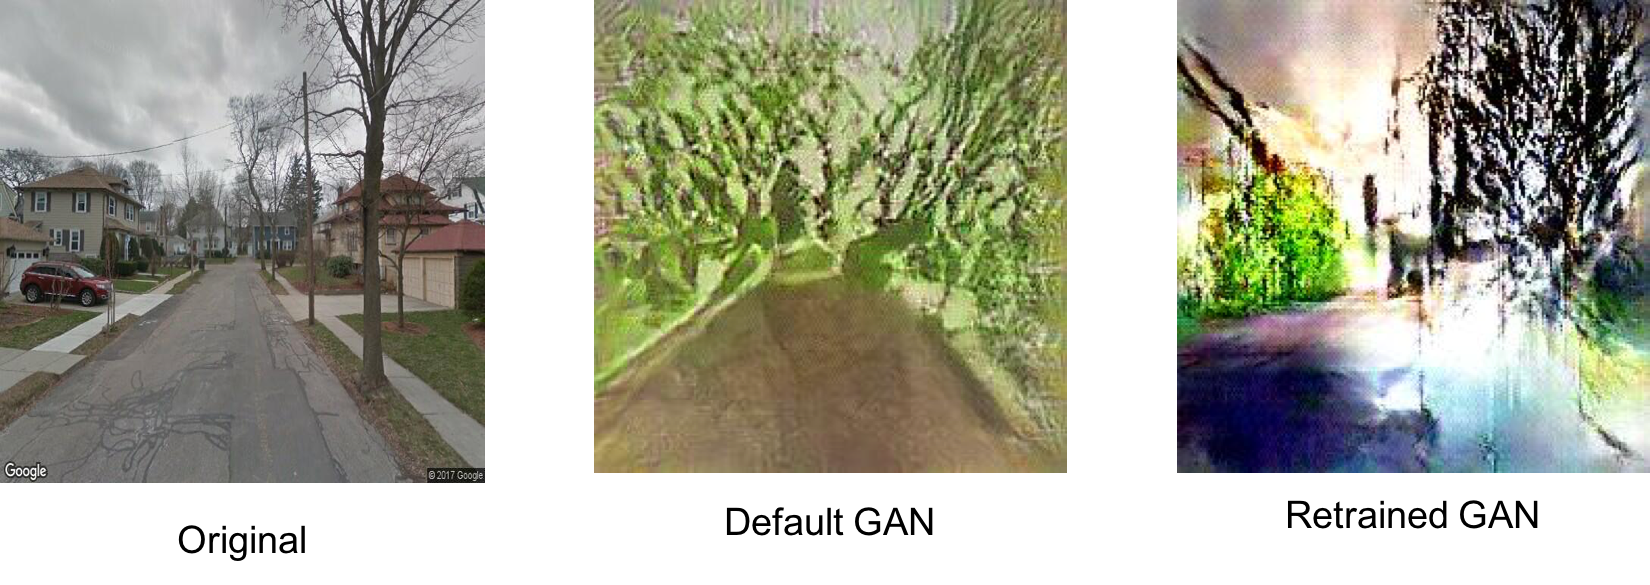
\includegraphics[width=0.5\linewidth]{Plot/GanCompare.png}
%	\caption{Comparison of using the Default ImageNet GAN against Custom trained GAN for Activation maximization. By re-training the GAN on the test dataset, we can see improvement in terms of structure and colours in the generated images}
%	\label{fig:GanComparison}
%\end{figure*}


%****************************************
\subsection*{Step 3 Generating a synthetic beautified scene}
Having this trained classifier at hand, we can then build a generator of synthetic beautified scenes. This is a model that, given the two classes ugly $y_i$ and beautiful $y_j$, transforms any original scene $I_i$ of class $y_i$ (e.g., ugly scene) into template scene $\hat{I_j}$ that maximizes class $y_j$ (e.g., beautified template scene). 

More specifically, given an input image $I_i$ known to be of class $y_i$  (e.g., ugly), our technique outputs  $\hat{I_j}$, which is a  more beautiful version of it (e.g., $I_i$ is morphed  towards the average representation of a beautiful scene) while preserving $I_i$'s details. The technique does so using the ``Deep Generator Network for Activation Maximization'' (\emph{DGN-AM}) \cite{nguyen2016synthesizing}. Given an input image $I_i$, \emph{DGN-AM} iteratively re-calculates the color of $I_i$'s pixels in  a way  the output image $\hat{I_j}$  both maximizes  the  activation of neuron $y_j$ (e.g., the ``beauty neuron'') and looks ``photo realistic'',  which is done by conditioning the maximization to an ``image prior''. This is equivalent to finding the feature vector $f$ that maximizes the following expression:
\begin{equation}
\hat{I_j} =G( f ) : \underset{f}{\arg\max}(C_{j}(G(f))-\lambda||f||)
\end{equation}
where:
\begin{itemize}
\item $G(f)$ is the image synthetically generated from the candidate feature vector $f$;
\item $C_j(G(f))$ is the activation value of neuron $y_j$ in the scene classifier $C$ (the value to be maximized);
\item $\lambda$ is a $L_2$ regularization term.
\end{itemize}
Here the initialization of $f$ is key. If $f$ were to be initialized with random noise, then the resulting $G(f)$ would be the average representation of category $y_j$ (of, e.g., beauty). Instead, since $f$ is initialized with $I_i$, then the resulting $G(f)$ is $I_i$'s version ``morphed to become more beautiful''. 
%Figure \ref{fig:BeautyExample} shows the activation maximization output in the center.

%****************************************
\subsection*{Step 4 Returning a realistic beautified scene}
 We now have template scene $\hat{I_j}$ (which is a synthetic beautified version of original scene $I_i$) and need to retrieve a realistic looking version of it. We do so by: \emph{i)} representing each of our original scenes in Step 1 (including $\hat{I_j}$) as a 4096 dimensional feature vector derived from the FC7 layer of  a pre-trained deep  network \cite{zhou2014learning}; \emph{ii)} computing the similarity (as $L_2$ Norm) between $\hat{I_j}$'s feature vector and each of the original scene's feature vector; and \emph{iii)} selecting the original scene most similar to $\hat{I_j}$. This results into the selection of the beautified scene $I_j$.
 
 
 %****************************************
\subsection*{Step 5 Identifying  characterizing urban elements}
Since original scene $I_i$ and beautified scene $I_j$ are real scenes and we make sure that they maintain the same structural characteristics (e.g., point of view, layout), we can easily compare them in terms of presence or absence of SegNet's and PlacesNet's labels. That is, we can determine how the original scene and its beautified version differ in terms of urban design elements. 
 
 
\begin{figure*}[h]
	\centering
	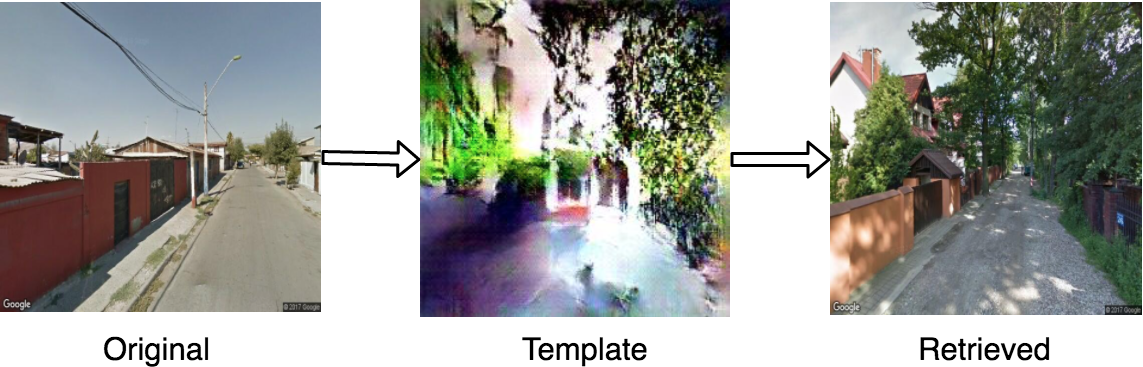
\includegraphics[width=\linewidth]{Plot/Example.png}
	\caption{Example of ``FaceLifting''.}
	\label{fig:BeautyExample}
\end{figure*}

